%
% "Building Debian Packages"
% Copyright (C) 2007  Chris Lamb <chris@chris-lamb.co.uk
% Based on a template (C) Daniel Watkins <D.M.Watkins@warwick.ac.uk>
%                         Chris Lamb <chris@chris-lamb.co.uk>
%
%  This program is free software; you can redistribute it and/or modify
%  it under the terms of the GNU General Public License as published by
%  the Free Software Foundation; either version 3 of the License, or
%  (at your option) any later version.
%
%  This program is distributed in the hope that it will be useful,
%  but WITHOUT ANY WARRANTY; without even the implied warranty of
%  MERCHANTABILITY or FITNESS FOR A PARTICULAR PURPOSE.  See the
%  GNU General Public License for more details.
%
%  You should have received a copy of the GNU General Public License
%  along with this program; if not, write to the Free Software
%  Foundation, Inc., 51 Franklin St, Fifth Floor, Boston, MA  02110-1301  USA

\documentclass{beamer}

\usepackage{beamerthemesplit}
\usetheme{Warsaw}

\usepackage{graphicx}
\usepackage{url} 

\usepackage{listings} 
\lstset{basicstyle=\ttfamily}


\title[Building Debian Packages]{Building Debian Packages}
\author[Chris Lamb, WUGLUG]{Chris Lamb\\Warwick University GNU/Linux User Group}
\date{7th November 2007
\newline
\newline

\includegraphics[width=15mm]{debian-logo.png}
\newline
\newline
\tiny{The \LaTeX{} source code for this presentation is licensed under version 3 of the GNU General Public License.}}

\begin{document}

\frame{\titlepage}

%%%%%%%%%%%%%%%%%%%%%%%%%%%%%%%%%%%%%%%%%%%%%%%%%%%%%%%%%%%%%%%%%%%%%%%%%%%%%%%%%%%%%%%%%%
\section{Packaging overview}

    \subsection{When to package}
        \frame {
            \frametitle{When to package}

            \begin{itemize}
                \pause
                \item Keeping your system 'clean'
                \pause
                \begin{itemize}
                    \item No `invisible' libraries 
                    \pause
                    \item Make upgrades easier
                    \pause
                    \item Works better with distributor packages
                \end{itemize}
                \pause
                \item Developing software:
                \begin{itemize}
                    \item \lstinline!/usr/local/! not really good enough
                \end{itemize}
            \end{itemize}
        }

    \subsection{When not to package}
        \frame {
            \frametitle{When not to package}

            \begin{itemize}
                \pause
                \item Sofware already packaged
                \pause
                \item Can be generated by helper commands:
                \begin{itemize}
                    \pause
                    \item \lstinline!alien! makes a good job of simple RPMs (controversial!)
                    \pause
                    \item CPAN packages: \lstinline!dh-make-perl --build --notest --cpan \$PACKAGE!
                \end{itemize}
            \end{itemize}
        }

\section{Creating a simple package}

    \subsection{Overview}

    \frame {
        \frametitle{Overview}

        \begin{itemize}

            \item Most packages have two components:
            \begin{enumerate}
                \item An `upstream tarball' (\lstinline!.orig.tar.gz!)
                \begin{itemize}
                    \item Contains the source of the program
                \end{itemize}
                \pause
                \item A `patch' (\lstinline!diff.gz!)
                \begin{itemize}
                    \item Adds packaging metadata
                    \item Can modify the upstream tarball
                \end{itemize}
            \end{enumerate}
        \end{itemize}
    }

    \frame {
        \center{ 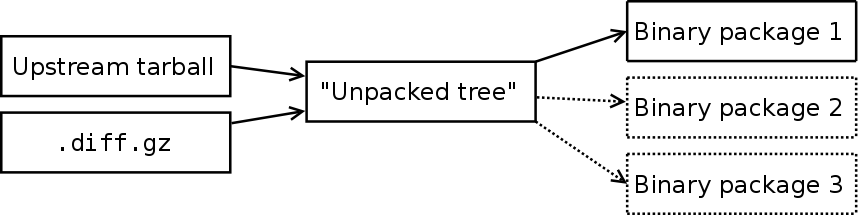
\includegraphics[width=105mm]{overview.png} }
    }

    \frame {
        \frametitle{The unpacked tree}
        \begin{itemize}
            \item Contains:
            \begin{itemize}
                \item Source code (and graphics, etc)
                \pause
                \item Packaging metadata
            \end{itemize}
            \vskip 1em
            \pause
            \item Packages can omit the patch - ``Debian native packages''
        \end{itemize}
    }

    \frame {
        \frametitle{Creating a package overview}
        \begin{itemize}
            \item To create a package:
            \begin{enumerate}
                \pause
                \item Obtain upstream tarball
                \pause
                \item Decompress
                \pause
                \item Add metadata via \lstinline!.diff.gz!
                \pause
                \item `Build' the source packages
                    \begin{itemize}
                        \item Generates patch against upstream tarball
                    \end{itemize}
                \pause
                \item `Build' the binary packages
            \end{enumerate}
            \pause
            \item The last two steps are usually performed together
        \end{itemize}
    }

    \subsection{Packaging metadata}
    \frame {
        \frametitle{Packaging metadata}
        \begin{itemize}
            \item All metadata resides below \lstinline!debian/!
            \pause
            \item Best practice not to modify outside of \lstinline!debian/!
            \pause
            \item Important files:
            \pause
            \begin{itemize}
                \item \lstinline!debian/control!
                \item \lstinline!debian/changelog!
                \item \lstinline!debian/copyright!
                \item \lstinline!debian/rules!
            \end{itemize}
        \end{itemize}
    }

    \frame {
        \frametitle{\lstinline!debian/control!}
        \begin{itemize}
            \item Contains build- and package-dependencies
            \pause
            \item Consists of:
            \begin{itemize}
                \item One \emph{source} stanza (build dependencies, `sections')
                \item One or more \emph{binary} stanzas (install dependencies)
            \end{itemize}
            \center{ 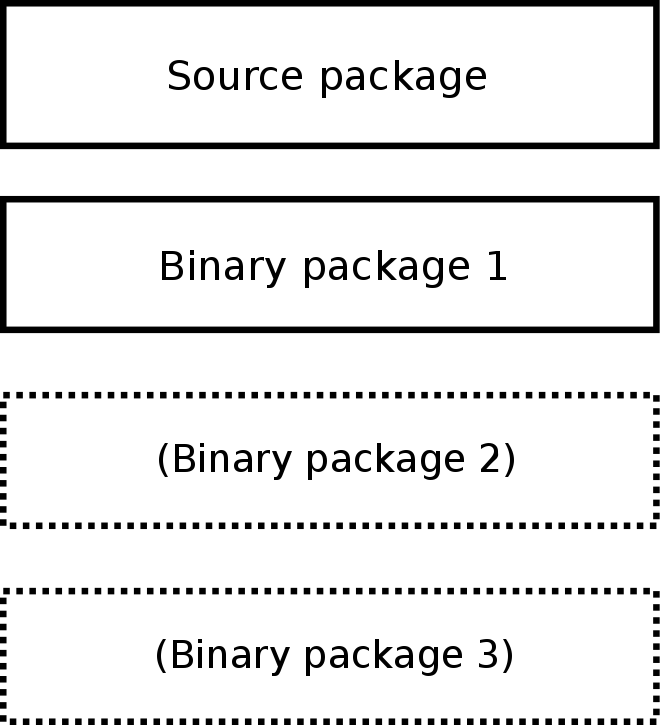
\includegraphics[width=20mm]{control.png} }
            \pause
            \item Names of source and binary packages in different namespaces
        \end{itemize}
    }

    \frame {
        \begin{itemize}
            \item Typical source stanza:
        \end{itemize}
        \begin{scriptsize}
            \lstinputlisting{control-source.txt}
        \end{scriptsize}
    }

    \frame {
        \begin{itemize}
            \item Typical binary stanzas (some omitted):
        \end{itemize}
        \begin{scriptsize}
            \lstinputlisting{control-binary.txt}
        \end{scriptsize}
    }

    \frame {
        \frametitle{\lstinline!debian/changelog!}
        \begin{itemize}
            \item Consists of: 
                \begin{itemize}
                    \pause
                    \item Source package name
                    \pause
                    \item Source package version
                    \pause
                    \item Source package distribution and urgency
                    \pause
                    \item What changed in this version (Trac-like bug closing)
                \end{itemize}
            \pause
            \item Picky format
            \pause
            \item Create entries with \lstinline!dch! tool
        \end{itemize}
    }

    \frame {
        \begin{tiny}
            \lstinputlisting{changelog.txt}
        \end{tiny}
    }

    \frame {
        \frametitle{\lstinline!debian/rules!}
        \begin{itemize}
            \item Responsible for compiling/assembling package
            \pause
            \item `Just' a Makefile
            \pause
            \item Targets specified in Debian Policy manual
            \pause
            \item Many approaches:
            \pause
            \begin{itemize}
                \item Building packages by hand (not recommended)
                \pause
                \item Debhelper (good)
                \pause
                \item CDBS (good, but controversial)
            \end{itemize}
        \end{itemize}
    }

    \frame {
        \frametitle{\lstinline!debian/rules! by hand}
        \begin{itemize}
            \item You shouldn't really build packages by hand
            \pause
            \item Quite educational
            \pause
        \end{itemize}

        \begin{scriptsize}
            \lstinputlisting{rules-byhand-1.txt}
        \end{scriptsize}
    }

    \frame {
        \begin{scriptsize}
            \lstinputlisting{rules-byhand-2.txt}
        \end{scriptsize}
    }

    \frame {
        \begin{scriptsize}
            \lstinputlisting{rules-byhand-3.txt}
        \end{scriptsize}
    }

    \frame {
        \begin{tiny}
            \lstinputlisting{rules-byhand-4.txt}
        \end{tiny}
    }

    %
    \frame {
        \frametitle{\lstinline!debian/rules! using Debhelper}
        \begin{itemize}
            \item Consists 50 helper scripts for common tasks
            \pause
            \item Packaging `toolbox'
            \pause
            \item Recommended method:
            \begin{itemize}
                \item Well-known
                \item Well-tested
                \item Well-maintained (Joey Hess)
            \end{itemize}
        \end{itemize}

        \begin{scriptsize}
            \lstinputlisting{rules-dh-1.txt}
        \end{scriptsize}
    }

    \frame {
        \begin{scriptsize}
            \lstinputlisting{rules-dh-2.txt}
        \end{scriptsize}
    }

    \frame {
        \begin{scriptsize}
            \lstinputlisting{rules-dh-3.txt}
        \end{scriptsize}
    }

    \frame {
        \begin{scriptsize}
            \lstinputlisting{rules-dh-4.txt}
        \end{scriptsize}
    }

    \frame {
        \frametitle{\lstinline!debian/rules! using CDBS}

        \begin{itemize}
            \item Includes pre-made Makefile (Blue Peter approach)
            \pause
            \item Results in very short \lstinline!debian/rules!
            \pause
            \item Controversial:
            \pause
            \begin{itemize}
                \item Buggy
                \pause
                \item Difficult to debug
                \pause
                \item Hides package building issues
                \pause
                \item Difficult to get sponsors
            \end{itemize}
            \pause
            \item Many `classes' for common packaging systems - Python \lstinline!distutils!, Haskell Cabal
            \pause
        \item Fine for well-tempered packages
        \end{itemize}
        \pause

        \begin{scriptsize}
            \lstinputlisting{cdbs.txt}
        \end{scriptsize}
    }

    \subsection{Building our first package}
    \frame {
        \frametitle{Building our package}

        \begin{block}{Using debuild}
            \lstinline!\$ debuild -uc -us!
        \end{block}

        \begin{itemize}
            \item Cleans environment variables
            \pause
            \item Calls \lstinline!dpkg-buildpackage!
            \pause
            \item Runs Lintian and Linda on resulting binary packages
            \pause
            \item Remove \lstinline!-uc -us! if you wish to sign your packages
            \pause
            \item Performs sanity checks
            \pause
            \item Many other methods (\lstinline!pbuilder!, \lstinline!qemubuilder!, \lstinline!cowbuilder!, etc.)
        \end{itemize}
    }

\section{Next steps}
    \subsection{Applying patches}
        \frame {
            \frametitle{Why apply patches to upstream?}

            \begin{itemize}
                \item Installs things in the wrong place
                \pause
                \item Doing things ``The \$DISTRIBUTION way''
                \pause
                \item Bugs in upstream build system
                \pause
                \item Bugs in upstream
                \pause
                \item Upstream may contain undistributable contents
            \end{itemize}
        }

        \frame {
            \frametitle{Methods for applying patches}
            \begin{itemize}
                \item Alter upstream tarball
                \pause
                \item Make alterations in unpacked source tree
                \pause
                \item Patch systems
                \pause
                \begin{itemize}
                    \item \lstinline!dpatch!
                    \pause
                    \item \lstinline!quilt!
                    \pause
                    \item Recommended method
                    \pause
                    \item Makes reading \lstinline!.diff.gz! difficult
                \end{itemize}
            \end{itemize}
        }

    \subsection{Building in a sane environment}
        \frame {
            \frametitle{Building in a sane environment}

            \pause
            \begin{itemize}
                \item Keep host system clean
                \pause
                \item Build for different architectures/distributions/releases
                \pause
                \item Prevents accidental linkage
                \pause
                \item Catches bugs in packaging
                \pause
                \item Reproducible builds
            \end{itemize}
         }

         \frame {
             \frametitle{Building in a sane environment}

             \begin{itemize}
                \item \lstinline!pbuilder! builds packages in a chroot
                \pause
                \item Provides wrappers to create and manage chroots
                \pause
                \item Simply replace \lstinline!debuild! with \lstinline!pdebuild!
                \pause
                \item \lstinline!qemubuilder! for ``native cross-compiling''
                \pause
                \item \lstinline!pbuilder-uml!
                \pause
             \end{itemize}

             \begin{block}{Backporting packages to Etch from Sid redux}
                \lstinline!\$ pbuilder --create --distribution etch! \\
                \lstinline!\$ apt-get source mypackage! \\
                \lstinline!\$ pdebuild!
             \end{block}
         }

    \subsection{Lintian and Linda}
        \frame {
            \frametitle{Lintian and Linda}

            \begin{itemize}
                \item Statically checks packages for common errors
                \pause
                \item Fairly comprehensive: spelling, executable stacks, encodings, etc.
                \pause
                \item Important that you fix errors
            \end{itemize}
            \pause
            \begin{block}{Dissecting a Lintian warning}
                \begin{itemize}
                    \item Check Lintian manual
                    \item Google
                    \item \begin{tiny}
                    \lstinline!dpkg -L lintian | grep "\^/usr/share/lintian/checks/" | xargs grep check-name!
                    \end{tiny}
                \end{itemize}
            \end{block}
        }

    \subsection{Sharing your packages}
        \frame {
            \frametitle{Sharing your packages}
            
            \begin{itemize}
                \item Distributing \lstinline!.deb!s vs. repositories
                \pause
                \item APT repository -- \lstinline!Packages! and \lstinline!Sources! files
                \pause
                \item Using \lstinline!dupload! to automate task
            \end{itemize}
        }

        \frame {
            \begin{scriptsize}
                \lstinputlisting{dupload.txt}
            \end{scriptsize}
        }

    \subsection{Other resources}
    \frame {
        \frametitle{Other resources}

        \begin{itemize}
            \item ``New Maintainers Guide'' -- \url{http://www.debian.org/doc/maint-guide/}
            \pause
            \item ``Ubuntu Packaging Guide'' -- \url{http://doc.ubuntu.com/ubuntu/packagingguide/C/}
            \pause
            \item ``New Packages - Debian Developers Reference'' -- \url{http://www.debian.org/doc/developers-reference/ch-pkgs.en.html\#s-newpackage}
            \pause
            \item ``Debian Mentors'' -- \url{http://mentors.debian.net}
            \pause
            \item Other packages -- \lstinline!apt-get source interesting-package!
        \end{itemize}
    }

%%%%%%%%%%%%%%%%%%%%%%%%%%%%%%%%%%%%%%%%%%%%%%%%%%%%%%%%%%%%%%%%%%%%%%%%%%%%%%%%%%%%%%%%%%

\frame {
    \frametitle{Thanks!}
    WUGLUG contact information:
    \begin{itemize}
        \item Website: \url{http://www.wuglug.org.uk}
        \item IRC: {\tt \#wuglug} on {\tt irc.uwcs.co.uk:6667}
        \item Mailing list: \url{https://mailman.warwickcompsoc.co.uk/listinfo/wuglug}
        \vskip 2em
        \item Talk next week: `Securing SSH' by Tim Retout.
    \end{itemize}
}

\end{document}
